La titolazione è una tipica operazione dell'analisi chimica che consiste nel determinare la concentrazione o \textbf{titolo} di una specie chimica in soluzione, facendola reagire con una quantità nota di un dato reagente, detto \textbf{titolante}.
\subsection{Titolazione acido forte-base forte}
Si versa in un beker dell'acido, si aggiungono una o al massimo due gocce di una soluzione di una soluzione che per ora chiamiamo \textit{indicatore}, che è un composto che cambia colore nell'istante in cui si passa da un PH ad un altro. Il cambio di colore prende il nome di \textit{viraggio dell'indicatore}.

Ci sono vari tipi di indicatore. Se volessimo osservare la fine della titolazione, ossia partiamo da una soluzione acida e aggiungiamo una base, è utile un indicatore che abbia un punto di viraggio per pH pari a 7. Non è necessario che l'indicatore cambi colore esattamente a quel pH, perché ci sarà un valore di pH acido superato il quale con appena qualche goccia di base si raggiunge l'equivalenza. Gli indicatori sono dunque delle sostanze che in modo visibile ai nostri occhi cambiano colore e ci danno indicazione sul cambiamento di pH.

Nello specifico, questa reazione conviene farla usando come indicatore una sostanza chiamata \textit{fenoltaleina}, o meglio soluzioni estremamente diluite (all'1\%) di questa. Basta mettere una goccia di questa soluzione nel beker per potere osservare un cambio di colore pressoché immediato. Quando?

In ambiente acido è incolore (quindi ad esempio partendo da una soluzione di acido cloridrico non vedremmo nulla), per pH tra 8.5 e 9 da incolore diventa rossa, quindi avremo l'indicazione che il pH ha raggiunto tale valore al cambio di colore della soluzione. Se avessimo voluto capire invece quando si aveva l'equivalenza (cioè pH=7), potremmo pensare di aver perso questo punto di equivalenza. Vedremo che non è così: in prossimità del punto di equivalenza il pH varierà in modo repentino, con piccolissime aggiunte; al contrario, quando si è lontani dal punti di equivalenza il pH cambierà molto poco pur aggiungendo, se partiamo da una soluzione acida, parecchia base. D'altronde, avendo definito il pH come il logaritmo dell'inverso della concentrazione degli ioni $\rm H_3O^+$ di una soluzione, ci aspettiamo un andamento logaritmico e non lineare per il pH dopo l'aggiunta di una base.

\vspace{0.2cm}Immaginiamo di avere due soluzioni in due bekere diversi. Nel primo abbiamo 100 mL di HCl 0.1-N (nota: per l'HCl normalità e molarità coincidono). Aggiungiamo in esso la prima goccia di indicatore e poi aggiungiamo lentamente NaOH 0.1-N\footnote{Ovviamente non è necessario scegliere stesse concentrazioni, le usiamo per comodità di calcolo.}. In questo caso, se partiamo da 100 mL di acido cloridrico 0.1-N, quando avremo aggiunto 100 mL di idrossido di sodio 0.1-N (quindi stessi volumi e stesse concentrazioni) non avremo più né acido né base perché si saranno neutralizzati totalmente formando cloruro di sodio:

$$\ce{HCl(aq) + NaOH(aq) -> NaCl(aq) + H_2O}$$

Va da ricordare che HCl acquoso, visto che si tratta di un acido forte, significa ione $\rm H_3O^+$ e ione $\rm Cl^-$ totalmente dissociati. Analogamente NaOH acquoso, visto che si tratta di una base forte, significa ione $\rm Na^+$ e ione $\rm OH^-$ totalmente dissociati.

\begin{center}
    \begin{tabular}{ccccccc}
        0.01 &  & 0.001 & & / & &\\
        HCl & + & NaOH & \ce{->} & NaCl & + & $\rm H_2O$\\
        0.009 &  &  / & & 0.001 & &\\
    \end{tabular}
\end{center}

\begin{center}
    \begin{tabular}{ccccccc}
        0.01 &  & 0.002 & & / & &\\
        HCl & + & NaOH & \ce{->} & NaCl & + & $\rm H_2O$\\
        0.008 &  &  / & & 0.002 & &\\
    \end{tabular}
\end{center}

\begin{center}
    \begin{tabular}{ccccccc}
        0.01 &  & 0.004 & & / & &\\
        HCl & + & NaOH & \ce{->} & NaCl & + & $\rm H_2O$\\
        0.006 &  &  / & & 0.004 & &\\
    \end{tabular}
\end{center}

\begin{center}
    \begin{tabular}{ccccccc}
        0.01 &  & 0.005 & & / & &\\
        HCl & + & NaOH & \ce{->} & NaCl & + & $\rm H_2O$\\
        0.005 &  &  / & & 0.005 & &\\
    \end{tabular}
\end{center}

\begin{center}
    \begin{tabular}{ccccccc}
        0.01 &  & 0.008 & & / & &\\
        HCl & + & NaOH & \ce{->} & NaCl & + & $\rm H_2O$\\
        0.002 &  &  / & & 0.008 & &\\
    \end{tabular}
\end{center}

\begin{center}
    \begin{tabular}{ccccccc}
        0.01 &  & 0.009 & & / & &\\
        HCl & + & NaOH & \ce{->} & NaCl & + & $\rm H_2O$\\
        0.001 &  &  / & & 0.009 & &\\
    \end{tabular}
\end{center}

\begin{center}
    \begin{tabular}{ccccccc}
        0.01 &  & $9.5 \cdot 10^{-3}$  & & / & &\\
        HCl & + & NaOH & \ce{->} & NaCl & + & $\rm H_2O$\\
        $5 \cdot 10^{-4}$ &  &  / & & $9.5 \cdot 10^{-3}$ & &\\
    \end{tabular}
\end{center}

\begin{center}
    \begin{tabular}{ccccccc}
        0.01 &  & $9.9 \cdot 10^{-3}$  & & / & &\\
        HCl & + & NaOH & \ce{->} & NaCl & + & $\rm H_2O$\\
        $1 \cdot 10^{-4}$ &  &  / & & $9.9 \cdot 10^{-3}$ & &\\
    \end{tabular}
\end{center}

\begin{center}
    \begin{tabular}{ccccccc}
        0.01 &  & $9.99 \cdot 10^{-3}$  & & / & &\\
        HCl & + & NaOH & \ce{->} & NaCl & + & $\rm H_2O$\\
        $1 \cdot 10^{-5}$ &  &  / & & $9.99 \cdot 10^{-3}$ & &\\
    \end{tabular}
\end{center}
\begin{center}
    \begin{tabular}{ccccccc}
        0.01 &  & $9.95 \cdot 10^{-3}$  & & / & &\\
        HCl & + & NaOH & \ce{->} & NaCl & + & $\rm H_2O$\\
        $5 \cdot 10^{-5}$ &  &  / & & $9.95 \cdot 10^{-3}$ & &\\
    \end{tabular}
\end{center}

\begin{center}
    \begin{tabular}{|p{1.5cm}|p{1.5cm}||p{1.5cm}|p{1.5cm}|}
        \textbf{pH} & \textbf{mL} & \textbf{pH} & \textbf{mL}\\
        1 & 0 & 2.59 & 95\\
        1.09 & 10 & 3.30 & 99\\
        1.18 & 20 & 3.60 & 99.5\\
        1.37 & 40 & 4.30 & 99.9\\
        1.48 & 50 & 4.60 & 99.95\\
        1.95 & 80 & 7 & 100\\
        2.28 & 90 &&\\
    \end{tabular}
\end{center}

\begin{figure}[H]
    \centering
    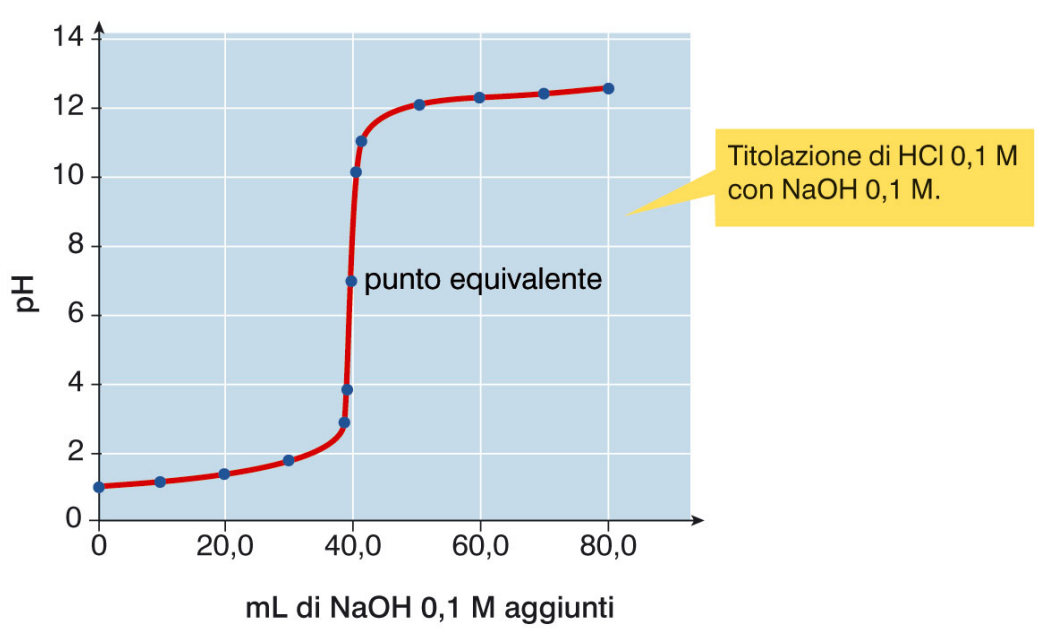
\includegraphics[width=14cm]{immagini/titolazione_acido_forte_base_forte.png}
\end{figure}

\subsection{Acidi deboli}

$$\ce{CH_3COOH(aq) + H_2O <--> CH_3COO^-(aq) + H_3O^+(aq)}$$

$$k_a=\frac{\rm{[CH_3COO^-]} \cdot \rm{[H_3O^+]}}{\rm{[CH_3COOH]}}$$

$$k_a=\frac{\rm{[H_3O^+]^2}}{\rm{[CH_3COOH]}}$$

\begin{center}
    \begin{tabular}{ccccccc}
        1 &  &  & & / & &\\
        $\rm CH_3COOH(aq)$ & + & $\rm H_2O$ & \ce{<-->} & $\rm CH_3COO^-(aq)$ & + & $\rm H_3O^+$\\
        $1-x$ & & & & $x$ & & $x$\\
    \end{tabular}
\end{center}

$$k_a = \frac{x^2 \, c^2}{(1-x)c}= c \frac{x^2}{(1-x)}$$

$$[\text{H}_3\text{O}^+]^2= k_a \cdot c_a$$

$$\implies [\text{H}_3\text{O}^+] = \sqrt{k_a \cdot c_a}$$

\subsection{Basi deboli}

$$\ce{NH_4OH <--> NH_4^+ + OH^-}$$

$$\ce{NH_3 \cdot H_2O <--> NH_4^+ + OH^-}$$

$$k_b= \frac{\rm{[NH_4^+] \cdot [OH^-]}}{\rm{[NH_3 \cdot H_2O]}}$$

$$k_b= \frac{\rm{[OH^-]^2}}{\rm{[NH_3 \cdot H_2O]}}$$

$$\implies \rm [OH^-] = \sqrt{ \textit{k}_{\textit{b}} \cdot [NH_3 \cdot H_2O]}$$

$$\implies  [\text{OH}^-] = \sqrt{ k_b \cdot c_b}$$
\subsection{Reazioni di idrolisi}
Se mettiamo un cucchiaino di cloruro di sodio in acqua ciò che avviene è solo la dissociazione dell'NaCl in ione $\rm Na^+$ e $\rm Cl^-$, senza che questi subiscano reazioni successive:

$$\ce{NaCl(aq) -> Na^+(aq) + Cl^-(aq)}$$

Se anziché avere cloruro di sodio avessimo acetato di sodio $\rm CH_3COONa$ cosa succederebbe?

Questo composto in acqua si dissocia in ione acetato $\rm CH_3COO^-$ e ione $\rm Na^+$

$$\ce{CH_3COONa -> CH_3COO^-(aq) + Na^+(aq)}$$

Nota: mettiamo una singola freccia perché è un sale, e i sali solubili sono tutti elettroliti forti e pertanto totalmente dissociati.

Lo ione $\rm Na^+(aq)$ non darà luogo ad ulteriori reazioni perché in acqua si hanno ioni $\rm H_3O^+$ e ioni $\rm OH^-$. La specie NaOH non si potrà formare perché è una base forte quindi totalmente dissociata, cosa che porta lo ione $\rm Na^+$ e lo ione $\rm OH^-$ a non potersi riassociare.

Lo ione acetato $\rm CH_3COO^-$ invece è la base di un acido debole, per cui dà ulteriori reazioni. In particolare esso reagisce con una molecola d'acqua e dà un equilibrio (a differenza della prima reazione che è una dissociazione in cui non c'è equilibrio). Con tale reazione di equilibrio lo ione acetato strappa un protone all'acqua riformando l'acido acetico e lasciando ioni $\rm OH^-$

$$\ce{CH_3COO^-(aq) + H_2O <--> CH_3COOH(aq) + OH^-(aq)}$$

Si forma quindi un acido, ma la soluzione è basica. Queste reazioni sono dette di \textbf{idrolisi}, in particolare la reazione appena vista è detta \textbf{idrolisi basica}.

La soluzione sarà basica perché l'acido che si forma è indissociato, ma in soluzione abbiamo anche eccesso di ioni $\rm OH^-$.

Quello che sta succedendo è che mettiamo in acqua un sale che è neutro (l'acetato di sodio) e troviamo una soluzione che è basica. Questo discorso è tipico di tantissimi saponi: essi sono neutri finché sono lontani dall'acqua, ma appena li bagniamo la specie che si ottiene non è più neutra.

In sintesi: abbiamo messo in acqua un sale neutro, che essendo un elettrolita forte si dissocia totalmente, dando ione acetato e ione sodio. Quest'ultimo non fa nulla, resta $\rm Na^+(aq)$, ossia anche se ci sono ioni $\rm OH^-$ in soluzione non si avrà la formazione dell'NaOH perché quest'ultimo è una base forte, quindi è tutta dissociata e non può associarsi. Invece lo ione acetato che produciamo, che è la base coniugata di un acido debole, strappa un protone all'acqua, forma l'acido acetico e pertanto avremo un eccesso di ioni $\rm OH^-$.

Trattandosi di un equilibrio, scriviamo la costante di questo equilibrio $k_i$, che sta per \textit{costante di idrolisi}. Va da notare che potremmo scrivere $k_b$ perché abbiamo scoperto che l'acetato di sodio è una base, in quanto sviluppa un ambiente basico con eccesso di ioni $\rm OH^-$:

$$k_i = \rm{\frac{[CH_3COOH] [OH^-]}{[CH_3COO^-]}} \quad (*)$$

Tuttavia i testi non riportano questa costante, ma quella $k_a$ dell'acido acetico sì. Allora moltiplichiamo e dividiamo per la concentrazione degli ioni $\rm H_3O^+$:

$$k_i = \rm{\frac{[CH_3COOH] [OH^-]}{[CH_3COO^-]} \cdot \frac{[H_3O^+]}{[H_3O^+]}}$$

In tale espressione al numeratore compare il prodotto $\rm [OH^-] \cdot [H_3O^+]$, che è il prodotto ionico dell'acqua $k_w$ che vale $1.0 \cdot 10^{-14}$. Ciò che invece resta è uguale all'inverso della $k_a$ dell'acido acetico:

$$k_i = \frac{k_w}{k_a}$$

Torniamo adesso alla $(*)$. Se guardiamo la reazione di equilibrio ci accorgiamo che ogni ione acetato che si idrolizza produrrà una molecola di acido e uno ione $\rm OH^-$, ossia queste quantità saranno uguali, quindi possiamo scrivere una sola quantità al quadrato:

$$k_i = \rm{\frac{[OH^-]^2}{[CH_3COO^-]}} \implies [OH^-]= \sqrt{\textit{k}_\textit{i} \cdot [CH_3COO^-]}$$

cioè la concentrazione degli ioni $\rm OH^-$ è uguale alla radice di $k_i$ per la concentrazione dello ione acetato all'equilibrio.

Se però consideriamo la prima definizione di $k_i$ come il rapporto $k_w/k_a$, abbiamo che

$$k_i = \frac{k_w}{k_a} = \frac{10^{-14}}{1.8 \cdot 10^{-5}}=5.55 \cdot 10^{-10}$$

Quindi la costante della reazione di equilibrio è molto piccola. Ne segue che la reazione è spostata a destra quasi per niente, ovvero gli ioni acetato ad idrolizzarsi sono pochi:

$$\rm{\frac{[OH^-]^2}{[CH_3COO^-]}} \approx 5.55 \cdot 10^{-10}$$

\E allora lecito supporre che non si sia idrolizzato nessuno ione acetato e che quindi la concentrazione all'equilibrio è uguale alla concentrazione iniziale del sale di partenza (la concentrazione iniziale di ione acetato è uguale a quella iniziale del sale, dato che quest'ultimo si dissocia totalmente):

$$[\text{OH}^-]=\sqrt{k_i \cdot C_s}=\sqrt{\frac{k_w}{k_a}\cdot C_s}$$

\E quindi ribadito il fatto che la concentrazione degli ioni $\rm [OH^-]$ è determinata dal valore di $k_i$, e la concentrazione del sale influisce poco. Dunque a priori ci aspettiamo già certi valori di pOH, ossia visto che lo ione acetato che si riassocia è pochissimo avremo una scarsa produzione di ioni $\rm [OH^-]$, quindi ci aspettiamo un pH basso, vicino alla neutralità, circa 8.

Facciamo un esempio. Consideriamo 7.5432 grammi di acetato di sodio AcNa in 575 mL. avremo

$$\rm [OH^-]=\sqrt{\frac{1 \cdot 10^{-14}}{1.8 \cdot 10^{-5}}\cdot \frac{7.5432}{82.0343} \cdot \frac{1000}{575}}$$

\subsubsection{Calcolare le moli conoscendo il volume ma non la massa}
Supponiamo di prelevare 3 litri di ammoniaca gassosa a condizioni normali e di farli gorgogliare in 700 mL di soluzione finale. Se la quantità ci viene data in litri e non in grammi come calcoliamo la concentrazione?

Ricordiamo la legge dei volumi molari, la quale afferma che a condizioni normali una mole di un gas occuperà sempre, qualunque sia il gas, un volume di 22.414 litri. Dato che siamo in condizioni normali, avremo

$$n_{\text{NH}_3}=\frac{3 \, L}{22.414 \, L}$$

ciò vale per qualunque gas prelevato a condizioni normali. Se venisse invece prelevato a condizioni diverse, conoscendo pressione e temperatura avremo che
$$n=\frac{PV}{RT}$$
\subsection{Soluzioni tampone}
Queste soluzioni si chiamano così perché hanno la caratteristica di mantenere un pH quasi invariato anche se noi dall'esterno, dopo aver generato la soluzione, aggiungiamo piccole quantità di acido o di base.

Va da ricordare che facendo la titolazione ad un certo punto con una goccia di base siamo passati da pH 4.6 a pH 7 e con un'altra goccia ancora a pH 9.4, quindi piccole quantità di acido o di base possono far cambiare drasticamente il pH. Chiaramente se anziché gocce mettiamo millilitri la situazione è ancora più marcata. Questo soluzioni tampone però hanno la caratteristica di fissare il pH a precisi valori e farlo variare pochissimo anche se aggiungiamo acido o base dall'esterno.

Sono importantissime perché esistono delle reazioni che avvengono a precisi valori di pH, quindi se tale reazione avviene in un ambiente opportuno procede, altrimenti no. Può darsi che man mano che queste reazioni procedono generino ioni $\rm H_3O^+$ o ioni $\rm OH^-$, modificando il pH della soluzione e bloccandosi. Con la soluzione tampone ciò non avviene: il pH non viene modificato in modo rilevante.

Si chiama quindi soluzione tampone perché "tampona" le aggiunte esterne di acido o di base.

Ne esistono di due tipi:

\begin{itemize}
    \item Acido debole + suo sale con base forte
    (Es. acido acetico con acetato di sodio);
    \item Base debole + suo sale con acido forte
    (Es. ammoniaca con cloruro di ammonio).
\end{itemize}

\subsubsection{Soluzioni tampone di primo tipo}
Consideriamo l'equilibrio dell'acido acetico

$$\ce{CH_3COOH(aq) + H_2O <--> CH_3COO^-(aq) + H_3O^+(aq)}$$

e la dissociazione di un suo sale con base forte

$$\ce{CH_3COONa(aq) -> CH_3COO^-(aq) + Na^+(aq)}$$

Lo ione $\rm Na^+$ non subisce altre reazioni, lo ione acetato si: esso si idrolizza in acqua dando acido acetico e ioni $\rm OH^-$

$$\ce{CH_3COO^-(aq) + H_2O <--> CH_3COOH(aq) + H_3O^+(aq)}$$

Sebbene abbiamo scritto la reazione del sale, sappiamo che  nel momento in cui questo viene messo in acqua si dissocia totalmente, essendo un elettrolita forte. In altre parole tale reazione non è un equilibrio, mentre la prima e la terza sì. Nello stesso volume di soluzione in cui abbiamo messo acido acetico e acetato di sodio avremo pertanto due equilibri contemporanei. Non solo: ci accorgiamo che questi due equilibri sono interdipendenti in quanto coinvolgono le stesse speci chimiche. Infatti in una abbiamo acido acetico al primo membro e nell'altro lo abbiamo a secondo membro e viceversa in una abbiamo ione acetato a secondo membro e nell'altra a primo membro. Ne segue che se muoviamo un equilibrio si muoverà anche l'altro.

Perché è una soluzione tampone?

Immaginiamo che a questa soluzione già preparata mescoliamo una certa quantità di acido e una di acetato di sodio. Si hanno questi due equilibri e il sistema finale è all'equilibrio. Dall'esterno mettiamo un po' di acido cloridrico. Cosa succede?

Succede che gli ioni $\rm OH^-$ intervengono per neutralizzare gli ioni $\rm H^+$ derivanti dall'HCl che aggiungiamo. Siccome abbiamo sottratto ioni $\rm OH^-$ il secondo equilibrio si sposterà per riprodurli, ma ciò comporterà anche la produzione di altro acido acetico.

Immaginiamo ora invece di avere introdotto dell'idrossido di sodio dall'esterno. Quello che succederà è che gli ioni $\rm H_3O^+$ neutralizzano gli ioni $\rm OH^-$ dell'NaOH. Ne segue che l'equilibrio della prima reazione si sposta a destra per riprodurli, ma di conseguenza aumenta la concentrazione dello ione acetato, perché non lo avevamo consumato.

Questo è come funziona il meccanismo tampone. Calcoliamone il pH.

Avendo due equilibri tra loro interdipendenti

$$k_a = \rm{\frac{[CH_3COO^-] \cdot [H_3O^+]}{[CH_3COOH]}}$$

$$[\text{H}_3\text{O}^+] = k_a \rm{\frac{[CH_3COOH]}{[CH_3COO^-]}}$$

$$[\text{H}_3\text{O}^+] = k_a \frac{c_a}{c_s}$$

$${[\text{H}_3\text{O}^+]}=\textit{k}_\textit{a} \frac{c_a + \rm{[\text{H}_3\text{O}^+]}}{c_s - \rm{[\text{H}_3\text{O}^+]}}$$

$${[\text{H}_3\text{O}^+]}=\textit{k}_a \frac{c_a - {[\text{OH}^-]}}{c_s + \rm{[\text{OH}^-]}}$$

\subsubsection{Soluzioni tampone di secondo tipo}
Essa è formata da una base debole più un suo sale con acido forte. Un esempio di base debole è l'ammoniaca e un suo sale con acido forte è il cloruro di ammonio.

L'$\rm NH_3$ in acqua instaura un equilibrio con formazione dello ione ammonio e dello ione $\rm OH^-$ in soluzione; l'$\rm NH_4Cl$ si dissocia in ione ammonio e ione $\rm Cl^-$. Quest'ultimo è l'anione di un acido forte, pertanto anche se in acqua ci sono ioni $\rm H_3O^+$ non ci sarà l'associazione e quindi non succede nulla. Lo ione ammonio al contrario è il catione di una base debole. Esso in acqua dà luogo ad un equilibrio di idrolisi, formando la specie $\rm NH_3$ associata ad una molecola d'acqua più lo ione $\rm H_3O^+$.

In sintesi

$$\ce{NH_3 \cdot H_2O(aq) <--> NH_4^+(aq) + OH^-(aq)}$$

$$\ce{NH_4Cl(aq) -> NH_4^+(aq) + Cl^-(aq)}$$

$$\ce{NH_4^+ + 2H_2O <--> NH_3 \cdot H_20 + H_3O^+}$$

Questi sono gli equilibri presenti in una soluzione tampone formata da

$$k_b = \rm{\frac{[NH_4^+] \cdot [OH^-]}{[NH_3 \cdot H_2O]}}$$

$$[\text{OH}^-] = k_b \rm{\frac{[NH_3 \cdot H_2O]}{[NH_4^+]}}$$

$$[\text{OH}^-] = k_b \frac{c_b}{c_s}$$

\subsection{Titolazione acido debole-base forte}

\subsection{Titolazione base debole-acido forte}

\subsection{Indicatori}
L'indicatore indica una variazione di pH. \E un composto che a seconda di come si dissocia mostra una forma acida e una forma basica aventi colori diversi.

Chiamiamo l'indicatore HIn. \E una specie debole che si dissocia in $\rm H^+$ e $\rm In^-$ (ovviamente in acqua $\rm H^+$ si associa all'acqua dando $\rm H_3O^+$). Essendo una specie debole avremo una reazione di equilibrio di dissociazione e quindi una costante di equilibrio

$$\ce{HIn(aq) + H_2O <--> H_3O^+ + In^-}$$

$$k_{In}=\frac{\rm{[H_3O^+]} \cdot \rm{[In^-]}}{\rm{[HIn]}}\implies \rm{[H_3O^+]}=\textit{k}_{\textit{In}} \frac{\rm{[HIn]}}{\rm{[In^-]}}$$

%Ogni ione $\rm H_3O^+$ corrisponderà ad uno ione $\rm In^-$, pertanto possiamo scrivere la concentrazione degli ioni $\rm H_3O^+$ al quadrato

$$\implies \rm pH = log \left( \frac{1}{[H_3O^+]} \right) = log \left( \frac{1}{\textit{k}_{\textit{In}}} \right) + log \left( \frac{\rm{[In^-]}}{\rm{[HIn]}} \right)$$

$$\implies \rm pH= p\textit{k}_\textit{a} + log \left( \frac{\rm{[In^-]}}{\rm{[HIn]}} \right)$$

Noi stiamo aggiungendo un colorante, che colora la soluzione in modo diverso a seconda che si sia in ambiente acido o in ambiente basico. \E importante allora capire le quantità relative delle due forme colorate. Ad occhio nudo non riusciamo a vedere se uno dei due è in eccesso di un minimo: per vederlo è necessario che una delle due forme sia più abbondante dell'altra.

Di norma allora si immagina di essere in condizioni tali che una delle due sia almeno 10 volte più abbondante dell'altra. 
\subsection{Solubilità}
Quando mettiamo qualcosa in acqua non è detto che essa si sciolga del tutto. Dobbiamo quindi stare attenti a ragionare su soluzioni, non sospensioni. In altre parole, se abbiamo messo in acqua un qualunque composto chimico e non si è sciolto totalmente, dobbiamo filtrare la soluzione. Ciò che non si è sciolto resterà nel filtro, la soluzione limpida invece passerà dal filtro e la otterremo nel beker.

\E quindi importante capire che esiste una \textbf{solubilità} di ogni specie chimica. Essa varia da composto a composto, passando da qualche milligrammo per litro a quasi un chilogrammo per litro.

Esempi di ciò sono il nitrato di potassio e il solfuro di mercurio. Della prima specie a 100° C se ne sciolgono circa 850 grammi in un litro di soluzione, mentre la seconda è talmente insolubile che forse in soluzione si scioglie qualche molecola.

\E possibile scrivere degli equilibri di solubilità per tutte le speci, ma non li trattateremo.